% TODO: Fix the figure wrapping here
\newpage

\subsubsection{User defined configuration}

% \begin{figure}[htbp]
\begin{wrapfigure}{r}{0.5\textwidth}
    % \vspace{-50px}
    \centering
    \caption{YAML Schema}
    \label{fig:YAMLSchema}
    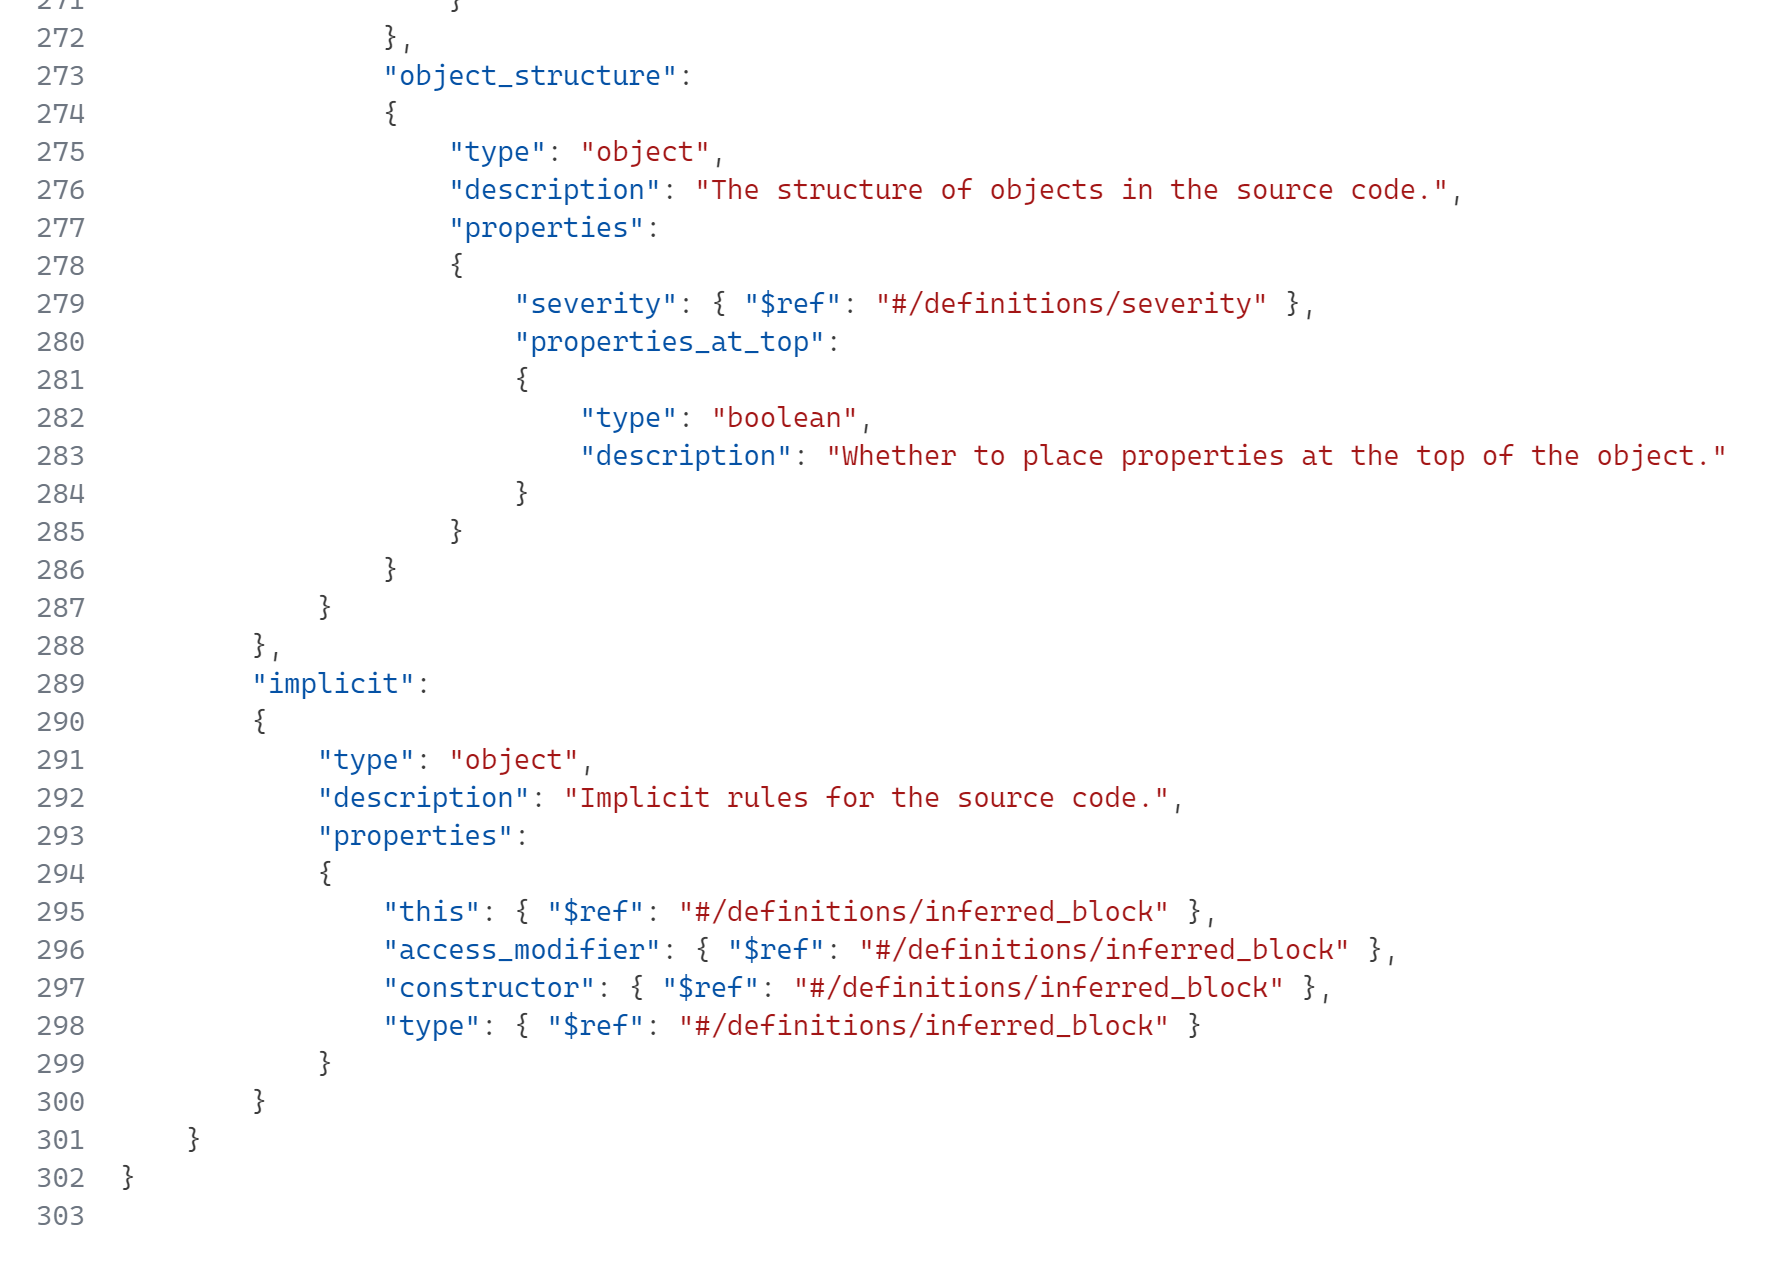
\includegraphics[width=0.5\textwidth]{Figures/YAMLSchemaCropped.png}
% \end{figure}
\end{wrapfigure}

% \begin{figure}[htbp]
%     \centering
%     \begin{minipage}[b]{0.5\textwidth}
%         \centering
%         \caption{YAML Schema}
%         \label{fig:YAMLSchema}
%         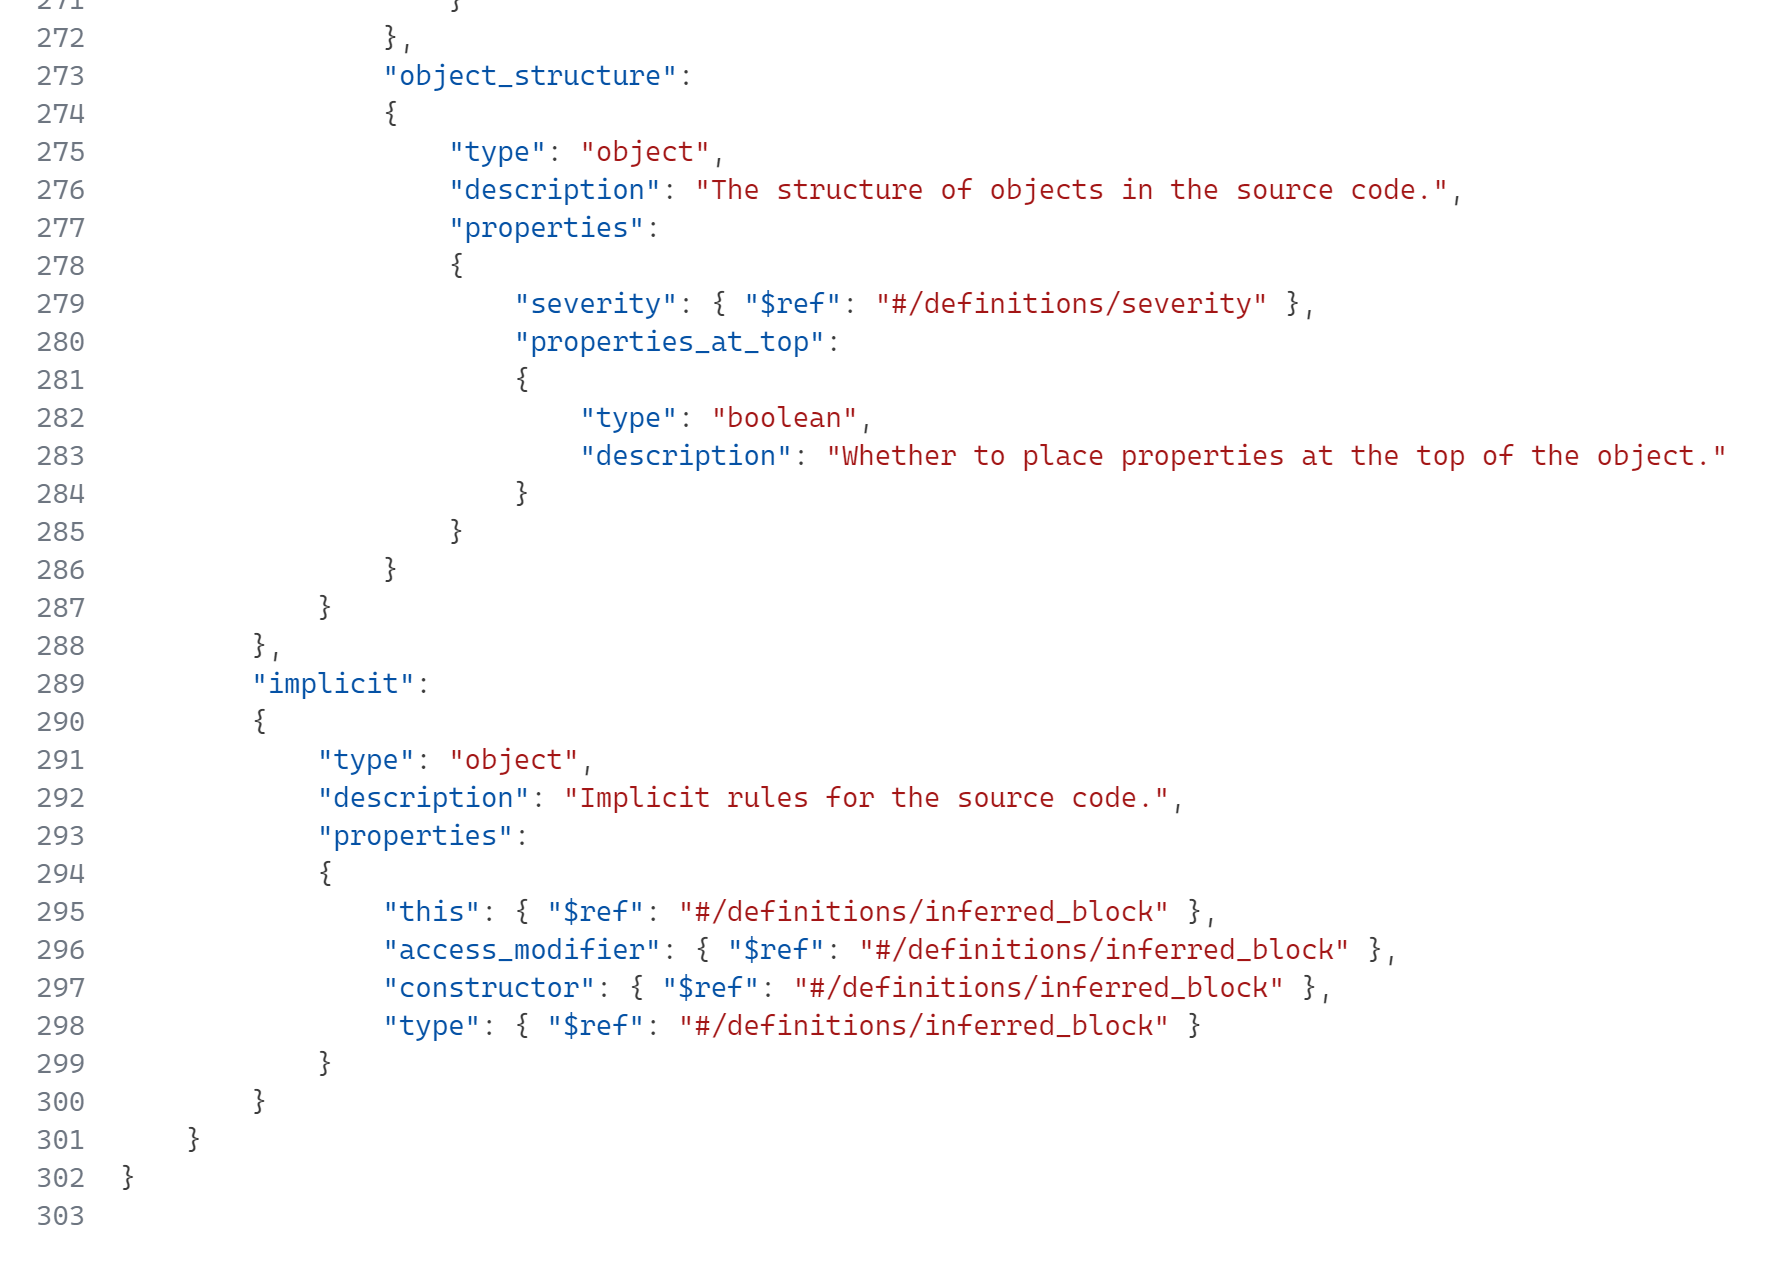
\includegraphics[width=0.5\textwidth]{Figures/YAMLSchemaCropped.png}
%     \end{minipage}
%     \hfill
%     \begin{minipage}[b]{0.4\textwidth}
%         \centering
%         \caption{YAML Configuration}
%         \label{fig:YAMLConfiguration}
%         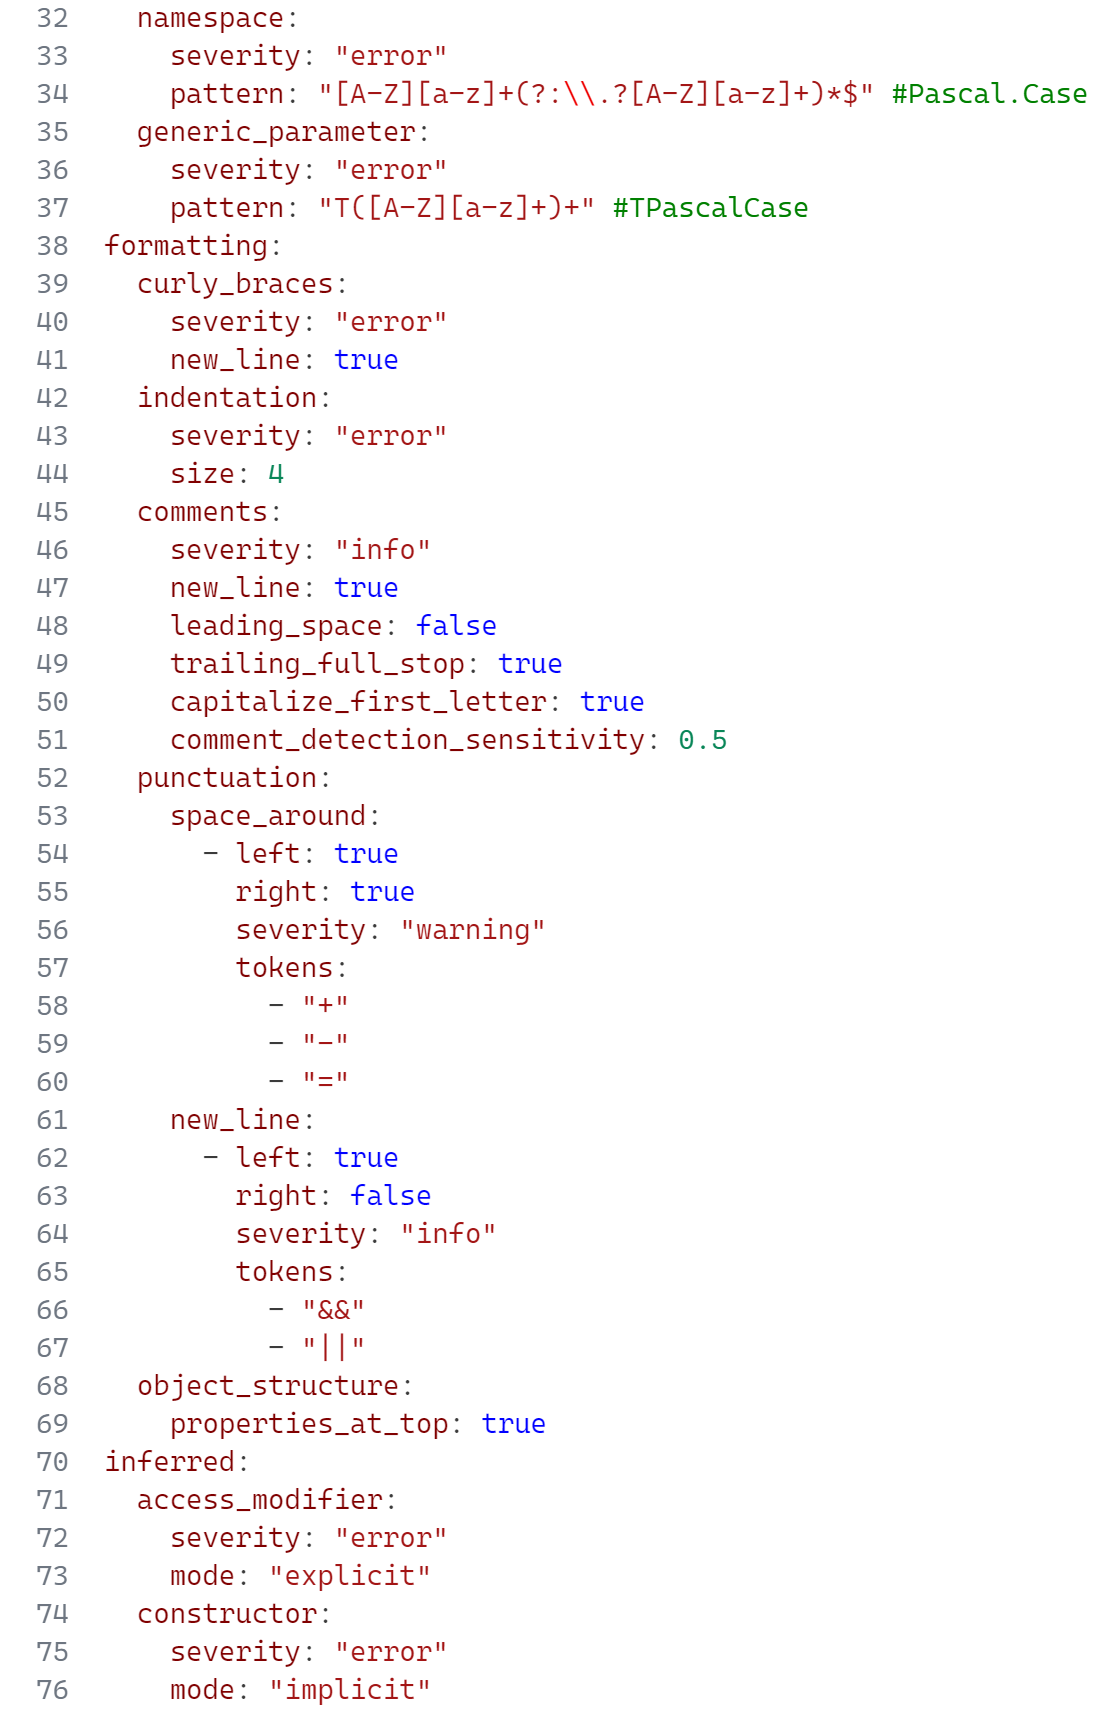
\includegraphics[width=0.4\textwidth]{Figures/YAMLConfigurationCropped.png}
%     \end{minipage}
% \end{figure}

As already noted, the lack of standardization in code formatting has lead to a key aim of this tool to be able to be configured by the user. It was also noted that this would be achieved through the use of a YAML configuration file. As configuration parsing isn't the goal of this work, the well-known, open source YAML parsing library YamlDotNet was used. This library is under the MIT license which grants full permission to use the library in this project.

YAML was chosen as the configuration language due to its human readability, as well as being very easy to implement and understand by the end user. A custom schema was created for the configuration to aid the user in creating the configuration file by providing IDE hints and validation on their configuration (see figure \ref{fig:YAMLSchema}).

\begin{wrapfigure}{r}{0.4\textwidth}
    \centering
    \caption{YAML Configuration}
    \label{fig:YAMLConfiguration}
    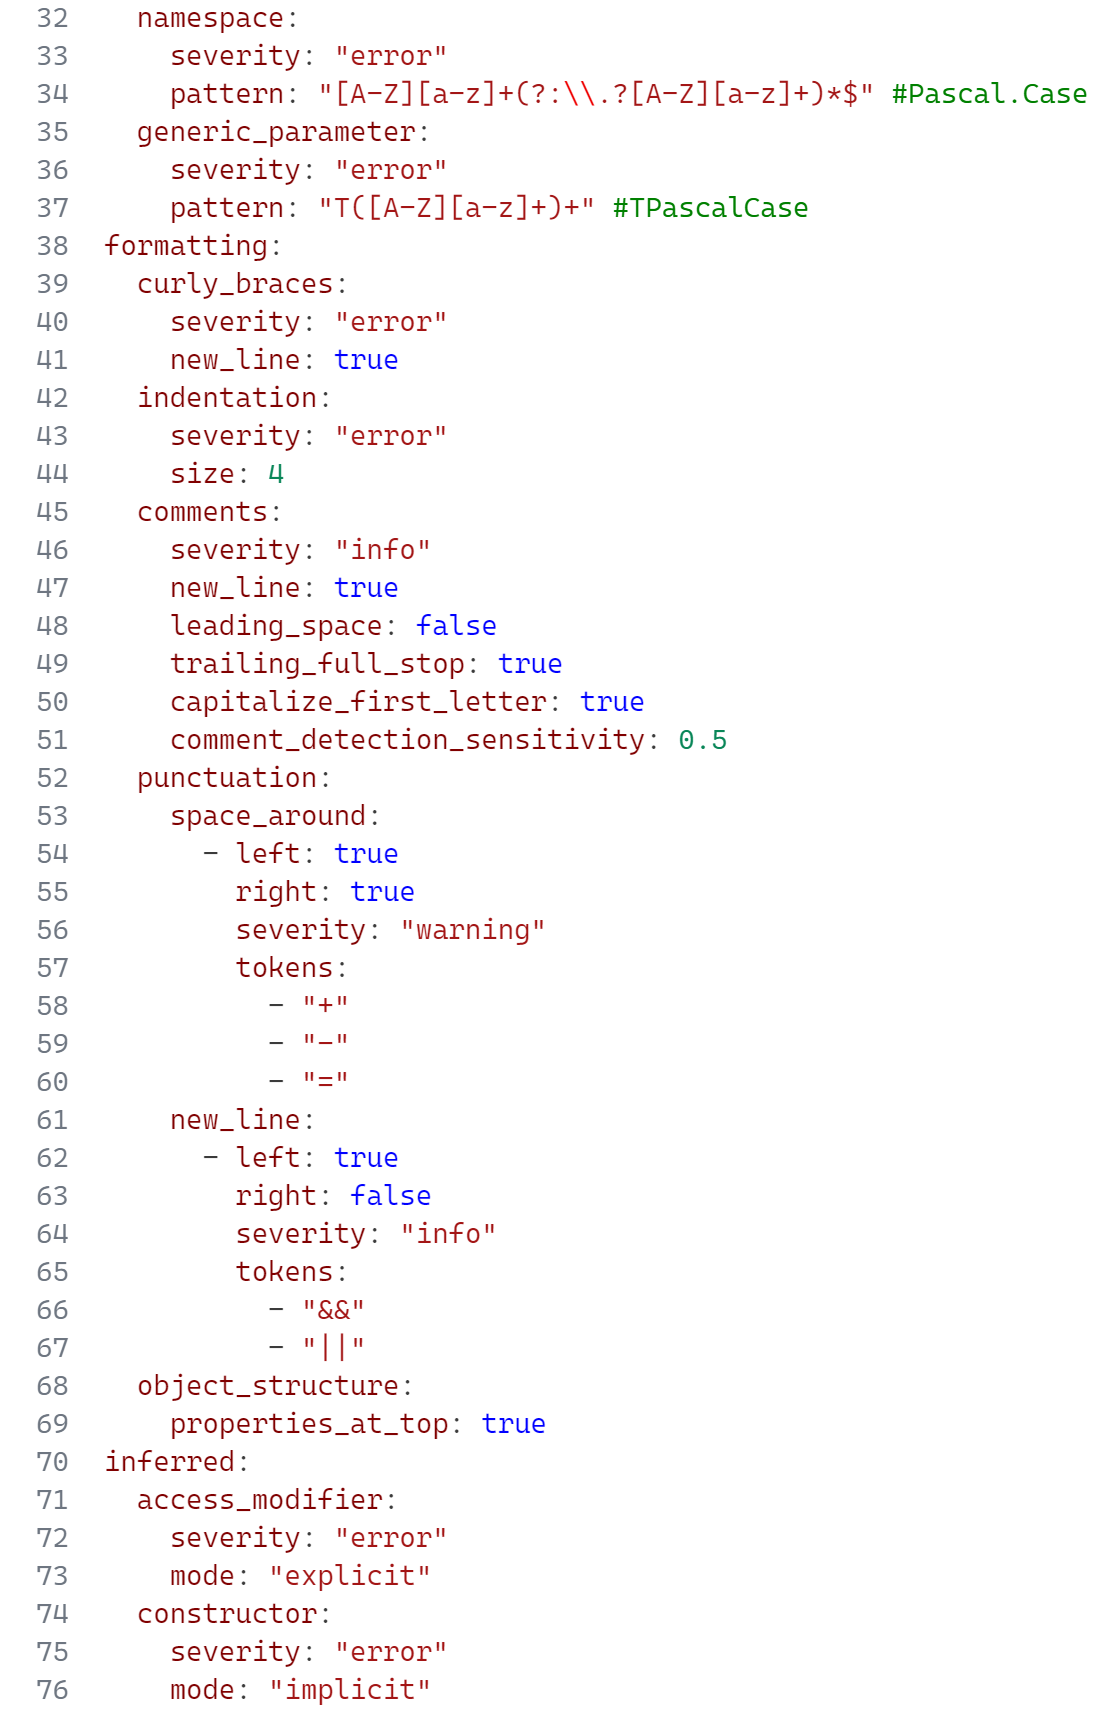
\includegraphics[width=0.4\textwidth]{Figures/YAMLConfigurationCropped.png}
\end{wrapfigure}

As with the program, the configuration is split up into multiple sections. Each section corresponds to a different module in the program with each module having a wide range of configuration options to allow for fine tuning of the program. In Figure \ref{fig:YAMLConfiguration} we can see an example of a configuration file, the visible snippet showing the configuration for the custom naming engine. Each module inherits from a base set of rules that allow the user to either enable or disable a module and set the severity of the issue that the module is checking for. By default, all modules are disabled and the severity is set to 'info'. Depending on how strict the work environment to be made, the severity can be set to cause an error which will result in not allowing the program to compile. This can be beneficial in a large team where you want to enforce a strict code style to improve readability and maintainability of the codebase.

The configuration file is loaded into the program at runtime. The way the configuration is loaded varies by the program implementing the tool due to the limitations of certain platforms, the configuration class has been created as a partial class that inherits from an interface where the configuration loader can be tweaked depending on the platform it is being compiled for. The configuration class is implemented as a singleton, as the code parser that is being used works in a static context, where configuration is loaded once and only once. This does have the downside of meaning any changes that the user wants to make to the configuration will require a restart of the program, which is a limitation of the Roslyn API and is not something that can easily be worked around.

\begin{wrapfigure}{r}{0.4\textwidth}
    \centering
    \caption{VSIX Configuration manager}
    \label{fig:VSIXConfigurationManager}
    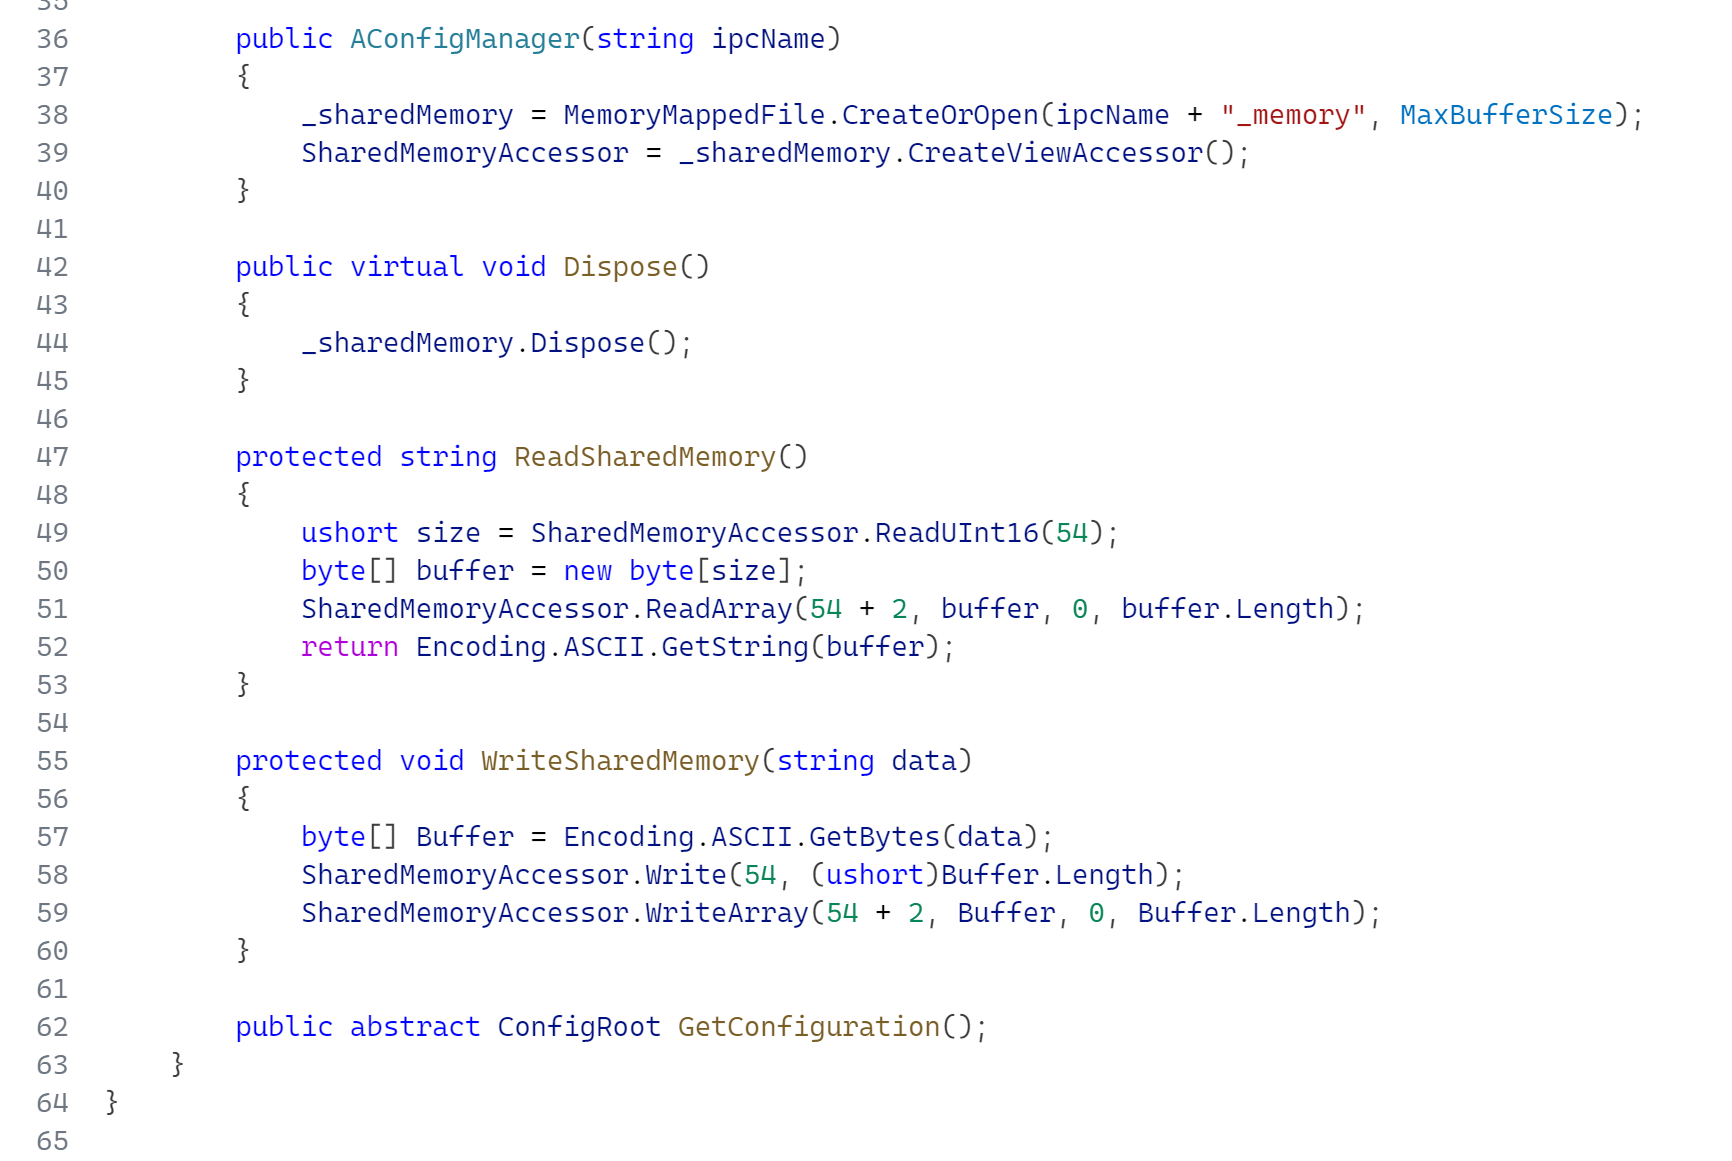
\includegraphics[width=0.4\textwidth]{Figures/VSIXAConfigManagerCropped.png}
\end{wrapfigure}

Taking the configuration implementation from the VSIX project as an example, the configuration is loaded when the extension is loaded into the IDE. The configuration also has to get loaded into a separate process that Visual Studio launches to run code analysis. This inherently caused a problem as it was discovered through debugging that the child-process does not have the context of the loaded workspace and so the user-defined configuration would not be found. To work around this issue, a shared memory space is setup between the two processes to allow for communication of the configuration to be shared (see figure \ref{fig:VSIXConfigurationManager}).
